\documentclass[main.tex]{subfiles} % Subfile-Class

%==============================================================================%
%                                   Subfile                                    %
%==============================================================================%

\begin{document}

% Template

\subsubsection{Chassis}

\subsubsection*{Anforderungen}

Die Anforderungen an das Chassis sind wesentlich geprägt durch die Limitationen 
hinsichtlich Gewicht und Budget sowie die hohen Ansprüche an die Funktionalität 
des Roboters. Das zulässige Gesamtgewicht stellt dabei eine besondere 
Herausforderung dar. Da bereits Akku, Motoren und elektronische Komponenten 
den Grossteil des Gewichtsbudgets beanspruchen, verbleiben lediglich \textbf{XXX} 
Gramm für das Chassis selbst. Diese Randbedingung verlangt nach einer besonders 
leichten, dennoch robusten und stabilen Konstruktion. Die Kosten sollen möglichst 
gering gehalten werden, indem die verfügbaren Ressourcen der Hochschule Luzern 
optimal genutzt werden. Konkret stehen dem Team 25 Stunden Druckzeit am 3D-Drucker 
zur Verfügung, welche maximal ausgeschöpft werden sollen, sodass das finanzielle 
Budget vor allem für funktionskritische Elemente wie die Greifeinheit 
und die Steuerung verwendet werden kann. Darüber hinaus müssen Stabilität und 
Zuverlässigkeit gewährleistet sein, um sicherzustellen, dass der Roboter den 
gegebenen Parcours vollständig autonom absolvieren kann.

\newpage

\subsubsection*{Konstruktive Umsetzung}

Das Chassis wurde vollständig aus PLA gefertigt und im 3D-Druckverfahren 
hergestellt. Im Gegensatz zum ursprünglichen Konzept aus PREN 1, in welchem 
MDF als Material für die Grundplatte vorgesehen war, bietet PLA die 
Möglichkeit, komplexere geometrische Formen und Strukturen direkt in einem 
einzigen Fertigungsschritt zu realisieren. Alle notwendigen Aussparungen 
und Montagelöcher wurden bereits während des Druckprozesses integriert, 
wodurch zusätzliche Bearbeitungsschritte entfallen und das Gewicht des 
Bauteils deutlich reduziert wird. Der Einsatz eines handelsüblichen 
3D-Druckers, welcher von einem Teammitglied bereitgestellt wurde, 
ermöglichte zudem eine flexible und zeitnahe Herstellung von Prototypen 
sowie eine iterative Umsetzung konstruktiver Verbesserungen. Für die Montage 
der Komponenten wurde eine kompakte Bauweise gewählt, die anstelle der 
bisherigen Etagenlösung auf einfache Distanzbolzen setzt. Dies verbessert die 
Zugänglichkeit der Komponenten erheblich, vereinfacht mögliche Anpassungen 
und trägt zusätzlich zur Gewichtsreduktion bei. Durch diese konstruktiven 
Massnahmen wurde eine ausgewogene Balance zwischen Stabilität, Gewicht und 
Kosten erzielt. Die finale Ausführung der Grundplatte ist in 
Abbildung~\ref{Chassis-Grundplatte} dargestellt.

\begin{figure}[H]
    \centering
    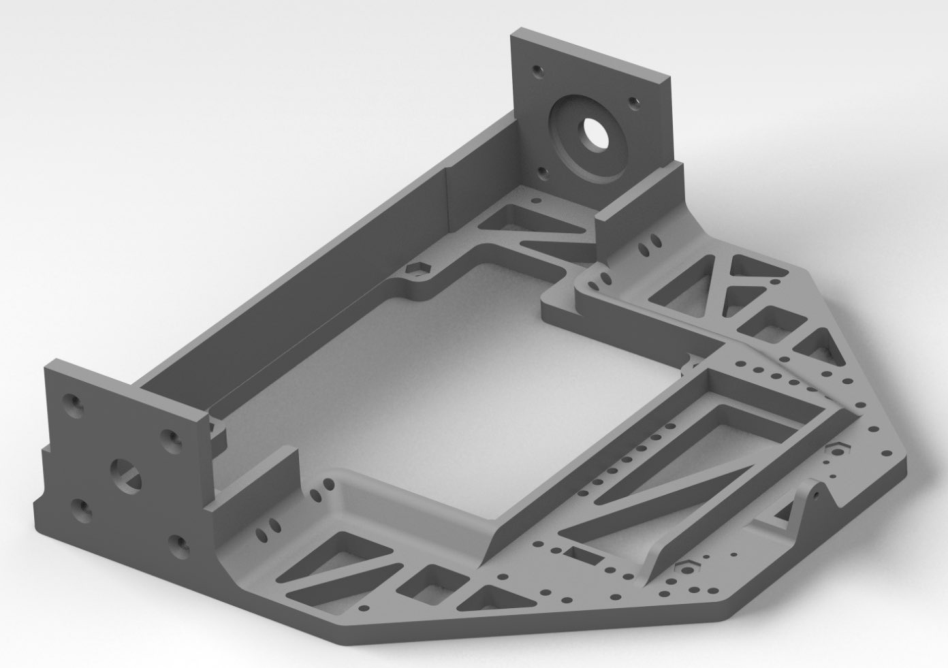
\includegraphics[width = 0.9\linewidth]{./fig_Mechanik/Rendering_Grundplatte.pdf}
    \caption{Rendering der Grundplatte in Siemens NX}~\label{Chassis-Grundplatte}
\end{figure}

\newpage

\subsubsection*{Fahrwerkskonzept}

Das Fahrwerkskonzept basiert auf einem Design mit zwei motorisch angetriebenen Rädern 
und einer Laufkugel, welche als dritter Auflagepunkt an der Fahrzeugfront dient. 
Diese Lösung zeichnet sich durch eine hohe Wendigkeit aus und ermöglicht präzise 
Kurskorrekturen sowie effiziente Drehmanöver auf den Knotenpunkten des Parcours. 
Die Positionierung der angetriebenen Räder an der Hinterachse sorgt nicht nur für eine 
verbesserte Traktion, sondern erlaubt auch schnelle und exakte Änderungen der 
Fahrzeugausrichtung.

Als Antriebsräder wurden Räder vom Typ FIT0500 von DFRobot mit einem Durchmesser von 
80 mm ausgewählt. Um die Umweltbelastung durch Einzelversand zu reduzieren, erfolgte 
der Bezug der Räder über eine Sammelbestellung der Hochschule Luzern. Mit diesen Rädern 
erreicht das Fahrzeug eine rechnerische Maximalgeschwindigkeit von etwa 1.676 m/s, 
welche sich nach folgender Formel berechnet:

\[ v_{max} = n_{Motor} \cdot d_{Rad} \cdot \pi = 1.676 \, \frac{\text{m}}{\text{s}} \]

Aus den eingekauften Rädern wurden schlussendlich nur die Reifen genutzt. Die 
Originalfelgen wurden durch speziell entwickelte Felgen ersetzt, welche im 
3D-Druckverfahren gefertigt wurden. Ein Detail der Eigenkonstruktion der Felgen zeigt 
Abbildung~\ref{Detailzeichnung-Felge}. Um eine optimale Auflagefläche des Reifens zu 
gewährleisten, wurde auf der Felgenaussenseite eine leichte Erhöhung integriert. Diese 
sorgt dafür, dass der Reifen über die gesamte Breite vollständig auf dem Boden aufliegt, 
wodurch der Grip erhöht wird. Die zentrale Aufnahme der Felge wurde präzise auf den 
Flansch der Motorenwelle abgestimmt und mittels einer Presspassung montiert, was eine 
besonders zuverlässige und spielfreie Verbindung ermöglicht. Das Felgendesign ist bewusst 
einfach gehalten und weist eine sternförmige Struktur mit zehn dünnen Speichen auf. Diese 
Konstruktion sorgt für eine ausgezeichnete Stabilität bei gleichzeitig minimalem Gewicht.

\begin{figure}[H]
    \centering
    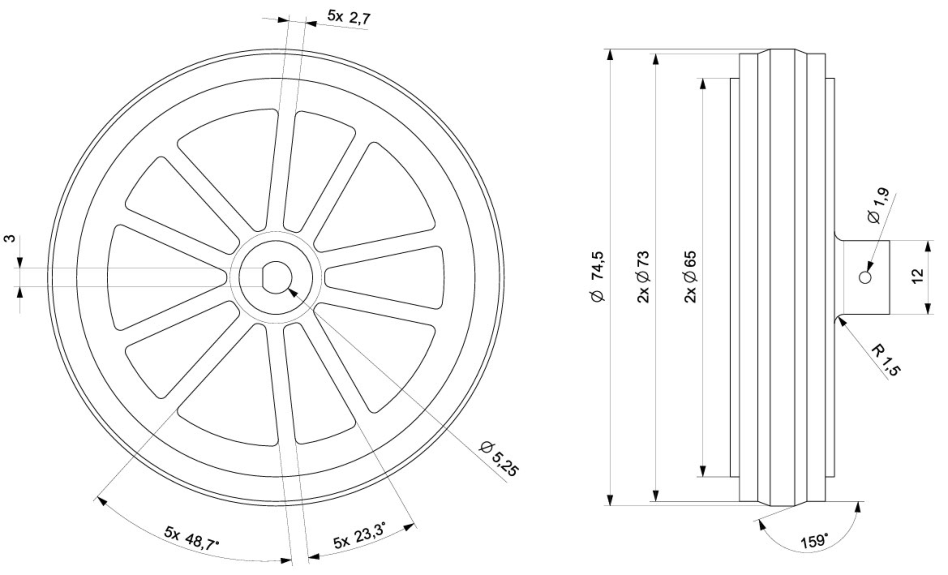
\includegraphics[width = 1\linewidth]{./fig_Mechanik/Detailzeichnung_Felge.pdf}
    \caption{Detailzeichnung der Felge in Siemens NX}~\label{Detailzeichnung-Felge}
\end{figure}

\end{document}
